\chapter{Arhitektura i dizajn sustava}
		
			Arhitektura sustava je web aplikacija kojoj će korisnici pristupati pomoću web preglednika. Odlučili smo se na takvu arhitekturu jer je cilj sustava da bude što jednostavniji za korištenje i da mu se može pristupiti sa svih mjesta.
			
			\begin{figure}[H]
				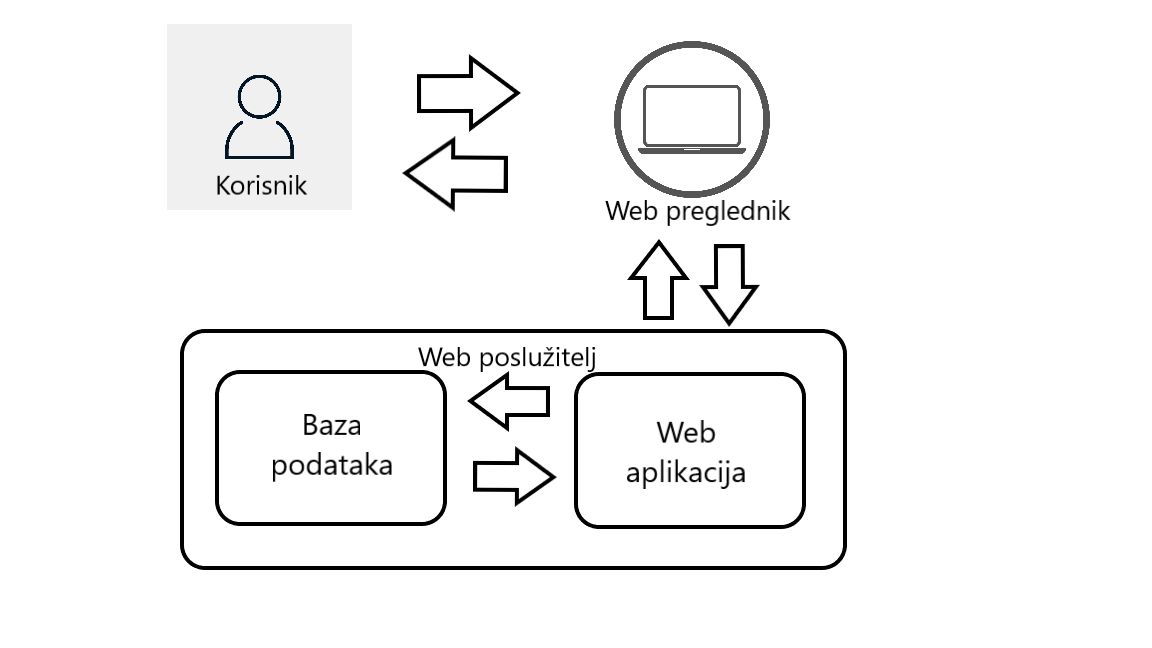
\includegraphics[scale=0.4]{slike/Skica_sustava.png} %veličina slike u odnosu na originalnu datoteku i pozicija slike
				\centering
				\caption{Skica sustava}
				\label{fig:sustav}
			\end{figure}
			
			Programski jezik koji smo odabrali za izradu aplikacije je Java s razvojnim okvirom Spring Boot te JavaScript. Odabrano razvojno okruženje je IntelliJ IDEA. 
			Aplikacija je organizirana u dva sloja: frontend i backend. Za izradu frontenda koristi se React - JavaScript biblioteka koja služi za izradu jednostraničnih aplikacija. Frontend i backend međusobno komuniciraju pomoću RESTa. REST se bazira na HTTP protokolu. Backend se sastoji od pet komponenti:
		\begin{itemize}
		\item Kontroler - služi za komunikaciju s frontendom. Zaprima HTTP zathtjev te određuje koja će se funkcionalnost izvršavati
		\item Servis - u njima se odvijaju poslovne logike i sve funkcionalnosti aplikacije
		\item Repozitorij - dohvaća i sprema podatke u bazu podataka
		\item Model - opisuju entitete iz baze 
		\item Security - omogućava autentikaciju i autorizaciju 
	\end{itemize}

\begin{figure}[H]
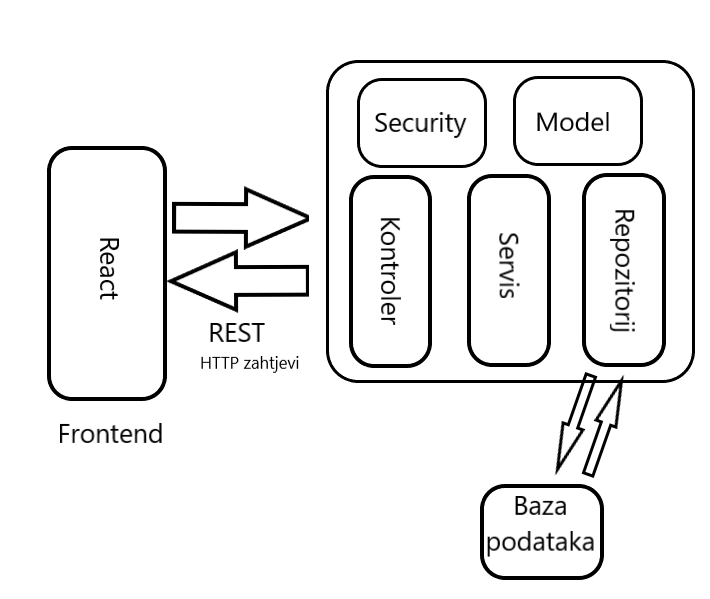
\includegraphics[scale=0.4]{slike/Skica_aplikacije.png} %veličina slike u odnosu na originalnu datoteku i pozicija slike
\centering
\caption{Skica aplikacije}
\label{fig:aplikacija}
\end{figure}


	
		

		

				
		\section{Baza podataka}
			
	Za potrebe sustava za zamjenu soba koristit ćemo relacijsku bazu podataka koja nam omogućuje oblikovanje objekata iz stvarnog svijeta pomoću povezanih tablica - relacija. Svaka je tablica definirana vlastitim nazivom i skupom različitih atributa koji je opisuju. Glavna je zadaća baze podataka pohrana, brzo pronalaženje i dohvaćanje te dodavanje i brisanje podataka. Baza podataka ovog sustava sastoji se od entiteta:
	\begin{itemize}
		\item Student
		\item Oglas
		\item Soba
		\item Grad
		\item Dom
		\item Paviljon
		\item StudentskiCentar
		\item Obavijest
		\item ZaposlenikSc
		\item TrazeniUvjeti
		\item Lajk
		\item StudentObavijesti
		\item Par
		\item Kandidat
		\item DomoviUvjeti
		\item PaviljoniUvjeti
		\item TrazeniUvjetiBrojKreveta
		\item TrazeniUvjetiKategorija
		\item TrazeniUvjetiKatovi
		\item TrazeniUvjetiTipKupaonice
		\\
		
	\end{itemize}
	
	\subsection{Opis tablica}
	
	Primarni ključevi entiteta u tablicama su označeni podebljanim fontom dok su strani ključevi označeni u nakošenom obliku.\\
	
	
	
	\textbf{Student } Entitet sadrži informacije o korisniku aplikacije - studentu. Sadrži sljedeće atribute: identifikator studenta, korisničko ime, JMBAG, ime, prezime, e-mail adresu, lozinku, oznaku za primanje mailova, hash kod lozinke, identifikator oglasa, identifikator grada i identifikator sobe. Entitet je u vezi \textit{Many-to-Many} s entitetom Obavijest preko identifikatora obavijesti,  u vezi \textit{One-to-One} s entitetom Oglas preko atributa identifikator oglasa, u vezi \textit{Many-to-One} s entitetom Grad preko atributa identifikator grada te u vezi \textit{One-to-One} s entitetom Soba preko identifikatora sobe.
	
	
	
	\begin{longtabu} to \textwidth {|X[6, 2]|X[6, 2]|X[20, l]|}
		
		\hline \multicolumn{3}{|c|}{\textbf{Student}}	 \\[3pt] \hline
		\endfirsthead
		
		\hline \multicolumn{3}{|c|}{\textbf{Student}}	 \\[3pt] \hline
		\endhead
		
		\hline
		\endlastfoot
		
		\textbf{idKorisnik} & UUID	& jedinstveni identifikator studenta (korisnika) 	\\ \hline
		korisnickoIme	& VARCHAR & jedinstveno korisničko ime  	\\ \hline
		jmbag & VARCHAR & jedinstveni JMBAG studenta \\ \hline
		ime & VARCHAR & ime studenta 		\\ \hline
		prezime & VARCHAR & prezime studenta \\ \hline
		email & VARCHAR & e-mail adresa studenta \\ \hline
		hashLozinke & VARCHAR & hash lozinka \\ \hline
		obavijestiNaMail & BOOLEAN & oznaka želi li student primati obavijesti na mail \\ \hline
%		\textit{idStatusOglasa} & BOOLEAN & oznaka potvrde \\ \hline
%		\textit{idTrazeniUvjeti} & VARCHAR & traženi kriteriji za sobu za zamjenu \\ \hline
		\textit{oglas} & UUID & identifikator studentovog oglasa \\ \hline
		\textit{idGrad} & UUID & identifikator grada u kojem student stanuje \\ \hline
		\textit{idSoba} & UUID & identifikator studentove sobe  
		
		
	\end{longtabu}
	
	\textbf{Oglas } Entitet sadrži informacije koje su vezane uz oglas koji student predaje. Sadrži atribute: ID oglasa, naslov oglasa, datum objave oglasa, status oglasa te identifikator sobe, identifikator studenta i identifikator traženih uvjeta. Entitet je u vezi \textit{One-to-One} s entitetom Student preko atributa identifiaktora studenta, u vezi \textit{One-to-Many} s entitetom Obavijest preko atributa identifikatora oglasa, u vezi \textit{One-to-Many} s entitetom Kandidat preko identifikatora kandidata oglasa, u vezi \textit{One-to-One} s entitetom Soba preko identifikatora sobe te u vezi \textit{One-to-One} s entitetom TrazeniUvjeti preko identifikatora traženih uvjeta.
	
	\begin{longtabu} to \textwidth {|X[6, 2]|X[6, 2]|X[20, l]|}
		
		\hline \multicolumn{3}{|c|}{\textbf{Oglas}}	 \\[3pt] \hline
		\endfirsthead
		
		\hline \multicolumn{3}{|c|}{\textbf{Oglas}}	 \\[3pt] \hline
		\endhead
		
		\hline
		\endlastfoot
		
		\textbf{idOglas} & UUID	& jedinstveni identifikator oglasa 	\\ \hline
		naslov & VARCHAR & naslov oglasa  	\\ \hline
		objavljen & DATE & datum objavljivanja oglasa 		\\ \hline
		statusOglasa & INTEGER & status oglasa \\ \hline
		\textit{idSoba} & UUID & identifikator sobe \\ \hline
		\textit{idStudent} & UUID & identifikator studenta \\ \hline
		\textit{idTrazeniUvjeti} & UUID & identifikator traženih uvjeta 
		
%		\textit{idStatusOglasa} & VARCHAR & status oglasa \\ \hline
		
		
		
		
	\end{longtabu}
	
	\textbf{Soba } Entitet sadrži informacije o sobi u studentskom domu. Sadrži atribute: identifikator sobe, kat na kojemu se soba nalazi, broj kreveta i vrsta kupaonice koja pripada sobi, dodatni komentar te identifikator paviljona i oglasa. Entitet je u vezi \textit{Many-to-One} s entitetom Paviljon preko atributa identifikator paviljona, u vezi \textit{One-to-One} s entitetom Oglas preko atributa identifikator oglasa te u vezi \textit{One-to-One} s entitetom Student preko identifikatora studenta.
	
	\begin{longtabu} to \textwidth {|X[6, 2]|X[6, 2]|X[20, l]|}
		
		\hline \multicolumn{3}{|c|}{\textbf{Soba}}	 \\[3pt] \hline
		\endfirsthead
		
		\hline \multicolumn{3}{|c|}{\textbf{Soba}}	 \\[3pt] \hline
		\endhead
		
		\hline
		\endlastfoot
		
		\textbf{idSoba} & INTEGER & identifikator sobe 	\\ \hline
		kat & INTEGER & kat na kojemu se soba nalazi \\ \hline
		brojKreveta & VARCHAR & broj kreveta u sobi \\ \hline
		tipKupaonice & VARCHAR & vrsta dostupne kupaonice \\ \hline
%		kategorija & VARCHAR & kategorija sobe \\ \hline
		komentar & TEXT & dodatni komentar o sobi \\ \hline
		\textbf{\textit{idPaviljon}} & UUID & identifikator paviljona kojemu soba pripada \\ \hline
%		\textbf{\textit{idDom}} & UUID & identifikator doma kojemu soba pripada \\ \hline
		\textit{idOglas} & UUID & identifikator oglasa 
		
		
	\end{longtabu}
	
	\textbf{Grad } Entitet sadrži informacije o pojedinom gradu. Sadrži atribute: identifikator grada i naziv te identifikator studentskog centra tog grada. Entitet je u vezi \textit{One-To-One} s entitetom Studentski Centar preko atributa identifikator studentskog centra, u vezi \textit{One-to-Many} s entitetom Dom preko identifikatora grada, u vezi \textit{One-to-Many} s entitetom TrazeniUvjeti preko identifikatora grada te u vezi \textit{One-to-Many} s entitetom Student preko identifikatora grada.
	
	\begin{longtabu} to \textwidth {|X[6, 2]|X[6, 2]|X[20, l]|}
		
		\hline \multicolumn{3}{|c|}{\textbf{Grad}}	 \\[3pt] \hline
		\endfirsthead
		
		\hline \multicolumn{3}{|c|}{\textbf{Grad}}	 \\[3pt] \hline
		\endhead
		
		\hline
		\endlastfoot
		
		\textbf{idGrad} & UUID	& jedinstveni identifikator grada	\\ \hline
		naziv	& VARCHAR & ime grada  	\\ \hline
		\textit{idSc} & UUID & identifikator gradskog studentskog centra 
		
		
	\end{longtabu}
	
	\textbf{Dom } Entitet sadrži sve važne informacije o pojedinom studentskom domu. Sadrži atribute: identifikator doma, naziv doma, identifikator grada u kojemu se dom nalazi te oznaka ima li dom vlastitu menzu. Entitet je u vezi \textit{Many-to-One} s entitetom Grad preko atributa identifikatora grada, u vezi \textit{One-To-Many} s entitetom Paviljon preko identifikatora doma te u vezi \textit{Many-to-Many} s entitetom TrazeniUvjeti. 
	
	\begin{longtabu} to \textwidth {|X[6, 2]|X[6, 2]|X[20, l]|}
		
		\hline \multicolumn{3}{|c|}{\textbf{Dom}}	 \\[3pt] \hline
		\endfirsthead
		
		\hline \multicolumn{3}{|c|}{\textbf{Dom}}	 \\[3pt] \hline
		\endhead
		
		\hline
		\endlastfoot
		
		\textbf{idDom} & UUID	& jedinstveni identifikator studentskog doma 	\\ \hline
		naziv	& VARCHAR & naziv studentskog doma  	\\ \hline
		imaMenzu & BOOLEAN & oznaka ima li dom vlastitu menzu \\ \hline
		\textit{idGrad} & UUID & identifikator grada u kojemu se dom nalazi 
		
		
	\end{longtabu}
	
	\textbf{Paviljon } Entitet sadrži sve informacije o pojedinom paviljonu studentskog doma. Sadrži atribute: identifikator paviljona, naziv, broj katova, kategorija u koju paviljon spada te identifikator doma. Entitet je u vezi \textit{Many-to-One} s entitetom Dom preko atributa identifikatoa doma,u vezi \textit{One-to-Many} s entitetom Soba preko indetifikatora paviljona te u vezi \textit{Many-to-Many} s entitetom TrazeniUvjeti.
	
	\begin{longtabu} to \textwidth {|X[6, 2]|X[6, 2]|X[20, 2]|}
		
		\hline \multicolumn{3}{|c|}{\textbf{Paviljon}}	 \\[3pt] \hline
		\endfirsthead
		
		\hline \multicolumn{3}{|c|}{\textbf{Paviljon}}	 \\[3pt] \hline
		\endhead
		
		\hline
		\endlastfoot
		
		\textbf{idPaviljon} & UUID	& jedinstveni identifikator paviljona	\\ \hline
		naziv & VARCHAR & naziv paviljona  	\\ \hline
		brojKatova & INTEGER & broj katova u paviljonu 	\\ \hline
		kategorija & VARCHAR & kategorija kojoj paviljon pripada 	\\ \hline
		\textit{idDom} & UUID & identifikator doma u kojemu se paviljon nalazi 
		
		
	\end{longtabu}
	
	
	\textbf{StudentskiCentar } Entitet sadrži informacije o studentskom centru. Sadrži atribute: identifikator studentskog centra, naziv te identifikator grada u kojemu se studentski centar nalazi. Entitet je u vezi \textit{One-to-One} s entitetom Grad preko atributa identifikatora grada te u vezi \textit{One-to-Many} s entitetom Zaposlenik SC preko identifikatora studentskog centra.
	
	\begin{longtabu} to \textwidth {|X[6, 2]|X[6, 2]|X[20, 2]|}
		
		\hline \multicolumn{3}{|c|}{\textbf{Studentski Centar}}	 \\[3pt] \hline
		\endfirsthead
		
		\hline \multicolumn{3}{|c|}{\textbf{Studentski centar}}	 \\[3pt] \hline
		\endhead
		
		\hline
		\endlastfoot
		
		\textbf{idSc} & UUID & jedinstveni identifikator studentskog centra	\\ \hline
		naziv  & VARCHAR & ime studentskog centra  	\\ \hline
		\textit{idGrad} & UUID & identifikator grada u kojemu se nalazi studentski centar
		
		
	\end{longtabu}
	
	\textbf{Obavijest} Entitet sadrži informacije o obavijestima koje aplikacija šalje studentima. Sadrži entitete: identifikator obavijesti, tekst, oznaka je li obavijest pročitana, vrijeme slanja obavijesti te lista studenata kojima se obavijest šalje i identifikator oglasa za koji se obavijest šalje. Entitet je u vezi \textit{Many-to-Many} s entitetom Student te u vezi \textit{Many-to-One} s entitetom Oglas preko identifikatora oglasa.
	
	\begin{longtabu} to \textwidth {|X[6, 2]|X[6, 2]|X[20, 2]|}
		
		\hline \multicolumn{3}{|c|}{\textbf{Obavijest}}	 \\[3pt] \hline
		\endfirsthead
		
		\hline \multicolumn{3}{|c|}{\textbf{Obavijest}}	 \\[3pt] \hline
		\endhead
		
		\hline
		\endlastfoot
		
		\textbf{idObavijest} & UUID & jedinstveni identifikator obavijesti	\\ \hline
		tekst  & VARCHAR & tekst obavijesti  	\\ \hline
		procitana & BOOLEAN & oznaka je li poruka pročitana \\ \hline
		vrijeme & DATE & vrijeme slanja obavijesti \\ \hline
		\textit{idOglas} & UUID & identifikator oglasa za koji se obavijest generira 
		
		
	\end{longtabu}
	
	\textbf{ZaposlenikSC } Entitet sadrži informacije o zaposleniku u studentskom centru. Sadrži atribute: identifikator zaposlenika, korisničko ime i lozinka za prijavu u sustav, ime i prezime zaposlenika, e-mail adresa, hash kod lozinke, oznaka o primanju obavijesti na e-mail te identifikator studentskog centra u kojem je zaposlen. Entitet je u vezi \textit{Many-to-One} s entitetom StudentskiCentar preko atributa identifikator studentskog centra.
	
	\begin{longtabu} to \textwidth {|X[6, 2]|X[6, 2]|X[20, 2]|}
		
		\hline \multicolumn{3}{|c|}{\textbf{ZaposlenikSc}}	 \\[3pt] \hline
		\endfirsthead
		
		\hline \multicolumn{3}{|c|}{\textbf{ZaposlenikSc}}	 \\[3pt] \hline
		\endhead
		
		\hline
		\endlastfoot
		
		\textbf{idZaposlenik} & UUID	& jedinstveni identifikator zaposlenika studentskog centra	\\ \hline
		korisnickoIme & VARCHAR & jedinstveno korisničko ime zaposlenika studentskog centra \\ \hline
		ime & VARCHAR & ime zaposlenika studentskog centra \\ \hline
		prezime & VARCHAR & prezime zaposlenika studentskog centra \\ \hline
		email & VARCHAR & e-mail adresa zaposlenika studentskog centra \\ \hline
		hashLozinke & VARCHAR & hash lozinke \\ \hline
		obavijestiNaMail & BOOLEAN & oznaka želi li zaposlenik primati obavijesti na mail \\ \hline
		\textit{idSc} & UUID & identifikator studentskog centra u kojemu je zaposlen 
		
		
		
	\end{longtabu}
	
	\textbf{TrazeniUvjeti} Entitet sadrži informacije o sobi koju student traži. Sadrži atribute: identifikator traženih uvjeta, identifikator grada i identifikator oglasa. Entitet je u vezi \textit{Many-to-One} s entitetom Grad preko identifikatora grada, u vezi \textit{Many-to-Many} s entitetom DomoviUvjeti te u vezi \textit{Many-to-Many} s entitetom PaviljoniUvjeti.
	
	\begin{longtabu} to \textwidth {|X[6, 2]|X[6, 2]|X[20, l]|}
		
		\hline \multicolumn{3}{|c|}{\textbf{TrazeniUvjeti}}	 \\[3pt] \hline
		\endfirsthead
		
		\hline \multicolumn{3}{|c|}{\textbf{TrazeniUvjeti}}	 \\[3pt] \hline
		\endhead
		
		\hline
		\endlastfoot
		
		\textbf{idTrazeniUvjeti} & UUID	& jedinstveni identifikator skupa traženih uvjeta	\\ \hline
		\textit{idGrad} & UUID & identifikator grada \\ \hline
		\textit{idOglas} & UUID & identifikator grada 
		
		
		
		
	\end{longtabu}
	
	\textbf{Lajk} Entitet sadrži informacije vezane uz 'lajkove' oglasa. Sadrži atribute: identifikator oglasa i identifikator studenta te ocjenu. Entitet je u vezi \textit{Many-to-One} s entitetom Student preko identifikatora studenta i u vezi \textit{Many-to-One} s entitetom Oglas preko identifikatora oglasa.
	
	\begin{longtabu} to \textwidth {|X[6, 2]|X[6, 2]|X[20, l]|}
		
		\hline \multicolumn{3}{|c|}{\textbf{Lajk}}	 \\[3pt] \hline
		\endfirsthead
		
		\hline \multicolumn{3}{|c|}{\textbf{Lajk}}	 \\[3pt] \hline
		\endhead
		
		\hline
		\endlastfoot
		
		\textbf{idOglas} & UUID & jedinstveni identifikator oglasa koji se ocjenjuje \\ \hline
		\textbf{idStudent} & UUID & jedinstveni identifikator studenta koji je 'dao lajk' \\ \hline
		ocjena & INTEGER & iznos ocjene 
		
		
	\end{longtabu}
	

	
	\textbf{StudentObavijesti } Entitet sadrži informacije vezane uz obavijesti i studente koji ih primaju. Sadrži atribute: identifikator studenta i identifikator obavijesti.
	
	\begin{longtabu} to \textwidth {|X[6, 4]|X[6, 2]|X[20, l]|}
		
		\hline \multicolumn{3}{|c|}{\textbf{StudentObavijesti}}	 \\[3pt] \hline
		\endfirsthead
		
		\hline \multicolumn{3}{|c|}{\textbf{StudentObavijesti}}	 \\[3pt] \hline
		\endhead
		
		\hline
		\endlastfoot
		
		\textit{studentiIdKorisnik} & UUID & identifikator studenta \\ \hline
		\textit{obavijestiIdObavijest} & UUID & identifikator oglasa 
		
	
	\end{longtabu}

	\textbf{Par } Entitet sadrži informacije vezane uz par za zamjenu sobe. Sadrži atribute: identifikator para, identifikator prvog oglasa u paru, identifikator drugog oglasa u paru, identifikator zaposlenika studentskog centra koji je potvrdio zamjenu te oznake statusa zamjene - done, ignore, lanac, odobren, prihvatio prvi, prihvatio drugi. Entitet je u vezi \textit{Many-to-One} s entitetom Oglas preko identifikatora oglasa za oba oglasa u paru te u vezi \textit{Many-to-One} s entitetom ZaposlenikSC.
	
	\begin{longtabu} to \textwidth {|X[6, 6]|X[6, 2]|X[20, l]|}
		
		\hline \multicolumn{3}{|c|}{\textbf{Par}}	 \\[3pt] \hline
		\endfirsthead
		
		\hline \multicolumn{3}{|c|}{\textbf{Par}}	 \\[3pt] \hline
		\endhead
		
		\hline
		\endlastfoot
		
		\textbf{idPar} & INTEGER & identifikator para  \\ \hline
		done & BOOLEAN & oznaka jesu li oba studenta prihvatila zamjenu \\ \hline
		ignore & BOOLEAN & oznaka je li barem jedan student odbio zamjenu \\ \hline
		lanac & BOOLEAN & oznaka je li zamjena nije obostrana nego ulančana \\ \hline
		odobren & BOOLEAN & oznaka je li djelatnik studentskog centra potvrdio zamjenu \\ \hline
		prihvatioDrugi & BOOLEAN & oznaka da je prvi student prihvatio zamjenu  \\ \hline
		prihvatioPrvi & BOLLEAN & oznaka da je drugi student prihvatio zamjenu \\ \hline
		\textit{idOglas1} & UUID & identifikator jednog oglasa u paru \\ \hline
		\textit{idOglas2} & UUID & identifikator drugog oglasa u paru \\ \hline
		\textit{zaposlenikKorisnickoIme} & UUID & identifikator zaposlenika studentskog centra koji je potvrdio zamjenu
		
		
		
	\end{longtabu}

	\textbf{Kandidat } Entitet sadrži informacije vezane uz mogućeg 'kandidata', to jest sobe za zamjenu. Sadrži atribute: identifikator kandidata, razinu bliskosti, oznake ignore i stvoren te identifikatore oglasa kandidata i oglasa za kojeg je pronađen kandidat. Entitet je u vezama \textit{Many-to-One} s entitetom Oglas preko identifikatora ogalsa i preko identifikatora kandidata oglasa.
	
	\begin{longtabu} to \textwidth {|X[6, 3.2]|X[6, 2]|X[20, l]|}
		
		\hline \multicolumn{3}{|c|}{\textbf{Kandidat}}	 \\[3pt] \hline
		\endfirsthead
		
		\hline \multicolumn{3}{|c|}{\textbf{Kandidat}}	 \\[3pt] \hline
		\endhead
		
		\hline
		\endlastfoot
		
		\textbf{idKandidat} & UUID & identifikator kandidata \\ \hline
		bliskost & INTEGER & broj zahtjeva koje oglas zadovoljava \\ \hline
		ignore & BOOLEAN & oznaka odbijanja kandidata \\ \hline
		stvoren & DATE & oznaka prihvata kandidata \\ \hline
		\textit{idKandOglasa} & UUID & identifikator oglasa kandidata \\ \hline
		\textit{idOglas} & UUID & identifikator oglasa za kojeg je pronađen kandidat
		
		
	\end{longtabu}

	\textbf{DomoviUvjeti } Entitet sadrži informaciju o domu za tražene uvjete. Sadrži atribute: identifikator doma i identifikator traženih uvjeta.
	
	\begin{longtabu} to \textwidth {|X[6, 4]|X[6, 2]|X[20, l]|}
		
		\hline \multicolumn{3}{|c|}{\textbf{DomoviUvjeti}}	 \\[3pt] \hline
		\endfirsthead
		
		\hline \multicolumn{3}{|c|}{\textbf{DomoviUvjeti}}	 \\[3pt] \hline
		\endhead
		
		\hline
		\endlastfoot
		
		\textbf{\textit{idDom}} & UUID & identifikator doma \\ \hline
		\textbf{\textit{idTrazeniUvjeti}} & UUID & identifikator traženih uvjeta 
		
		
		
	\end{longtabu}

	\textbf{PaviljoniUvjeti } Entitet sadrži informaciju o paviljonu za tražene uvjete. Sadrži atribute: identifikator paviljona i identifikator traženih uvjeta.
	
	\begin{longtabu} to \textwidth {|X[6, 4]|X[6, 2]|X[20, l]|}
		
		\hline \multicolumn{3}{|c|}{\textbf{PaviljoniUvjeti}}	 \\[3pt] \hline
		\endfirsthead
		
		\hline \multicolumn{3}{|c|}{\textbf{PaviljoniUvjeti}}	 \\[3pt] \hline
		\endhead
		
		\hline
		\endlastfoot
		
		\textbf{\textit{idPaviljon}} & UUID & identifikator paviljona \\ \hline
		\textbf{\textit{idTrazeniUvjeti}} & UUID & identifikator traženih uvjeta 
		
		
		
	\end{longtabu}

	\textbf{TrazeniUvjetiBrojKreveta} Entitet sadrži informaciju o broju kreveta za tražene uvjete. Sadrži atribute: broj kreveta i identifikator traženih uvjeta.
	
	\begin{longtabu} to \textwidth {|X[6, 10]|X[6, 2]|X[20, l]|}
		
		\hline \multicolumn{3}{|c|}{\textbf{TrazeniUvjetiBrojKreveta}}	 \\[3pt] \hline
		\endfirsthead
		
		\hline \multicolumn{3}{|c|}{\textbf{TrazeniUvjetiBrojKreveta}}	 \\[3pt] \hline
		\endhead
		
		\hline
		\endlastfoot
		
		brojKreveta & INTEGER & traženi broj kreveta \\ \hline
		\textit{trazeniUvjetiIdTrazeniUvjeti} & UUID & identifikator traženih uvjeta 
		
		
		
	\end{longtabu}

	\textbf{TrazeniUvjetiKategorija} Entitet sadrži informacije o kategoriji sobe za tražene uvjete. Sadrži atribute: kategorija i identifikator traženih uvjeta.
	
	\begin{longtabu} to \textwidth {|X[6, 10]|X[6, 2]|X[20, l]|}
		
		\hline \multicolumn{3}{|c|}{\textbf{TrazeniUvjetiKategorija}}	 \\[3pt] \hline
		\endfirsthead
		
		\hline \multicolumn{3}{|c|}{\textbf{TrazeniUvjetiKategorija}}	 \\[3pt] \hline
		\endhead
		
		\hline
		\endlastfoot
		
		kategorija & INTEGER & tražena kategorija sobe \\ \hline
		\textit{trazeniUvjetiIdTrazeniUvjeti} & UUID & identifikator traženih uvjeta 
		
		
		
	\end{longtabu}

	\textbf{TrazeniUvjetiKatovi} Entitet sadrži informaciju o katu na kojemu se nalazi soba za tražene uvjete. Sadrži atribute: katovi i identifikator traženih uvjeta.
	
	\begin{longtabu} to \textwidth {|X[6, 10]|X[6, 2]|X[20, l]|}
		
		\hline \multicolumn{3}{|c|}{\textbf{TrazeniUvjetiKatovi}}	 \\[3pt] \hline
		\endfirsthead
		
		\hline \multicolumn{3}{|c|}{\textbf{TrazeniUvjetiKatovi}}	 \\[3pt] \hline
		\endhead
		
		\hline
		\endlastfoot
		
		katovi & INTEGER & traženi kat na kojemu se nalazi soba \\ \hline
		\textit{trazeniUvjetiIdTrazeniUvjeti} & UUID & identifikator traženih uvjeta 
		
		
		
	\end{longtabu}

		\textbf{TrazeniUvjetiTipKupaonice} Entitet sadrži informaciju o tipu kupaonice za tražene uvjete. Sadrži atribute: tip kupaonice i identifikator traženih uvjeta.
	
	\begin{longtabu} to \textwidth {|X[6, 10]|X[6, 2]|X[20, l]|}
		
		\hline \multicolumn{3}{|c|}{\textbf{TrazeniUvjetiTipKupaonice}}	 \\[3pt] \hline
		\endfirsthead
		
		\hline \multicolumn{3}{|c|}{\textbf{TrazeniUvjetiTipKupaonice}}	 \\[3pt] \hline
		\endhead
		
		\hline
		\endlastfoot
		
		tipKupaonice & INTEGER & traženi tip kupaonice \\ \hline
		\textit{trazeniUvjetiIdTrazeniUvjeti} & UUID & identifikator traženih uvjeta 
		
		
		
	\end{longtabu}
	
	
	
	
	\subsection{Dijagram baze podataka}
	\begin{figure}[H]
		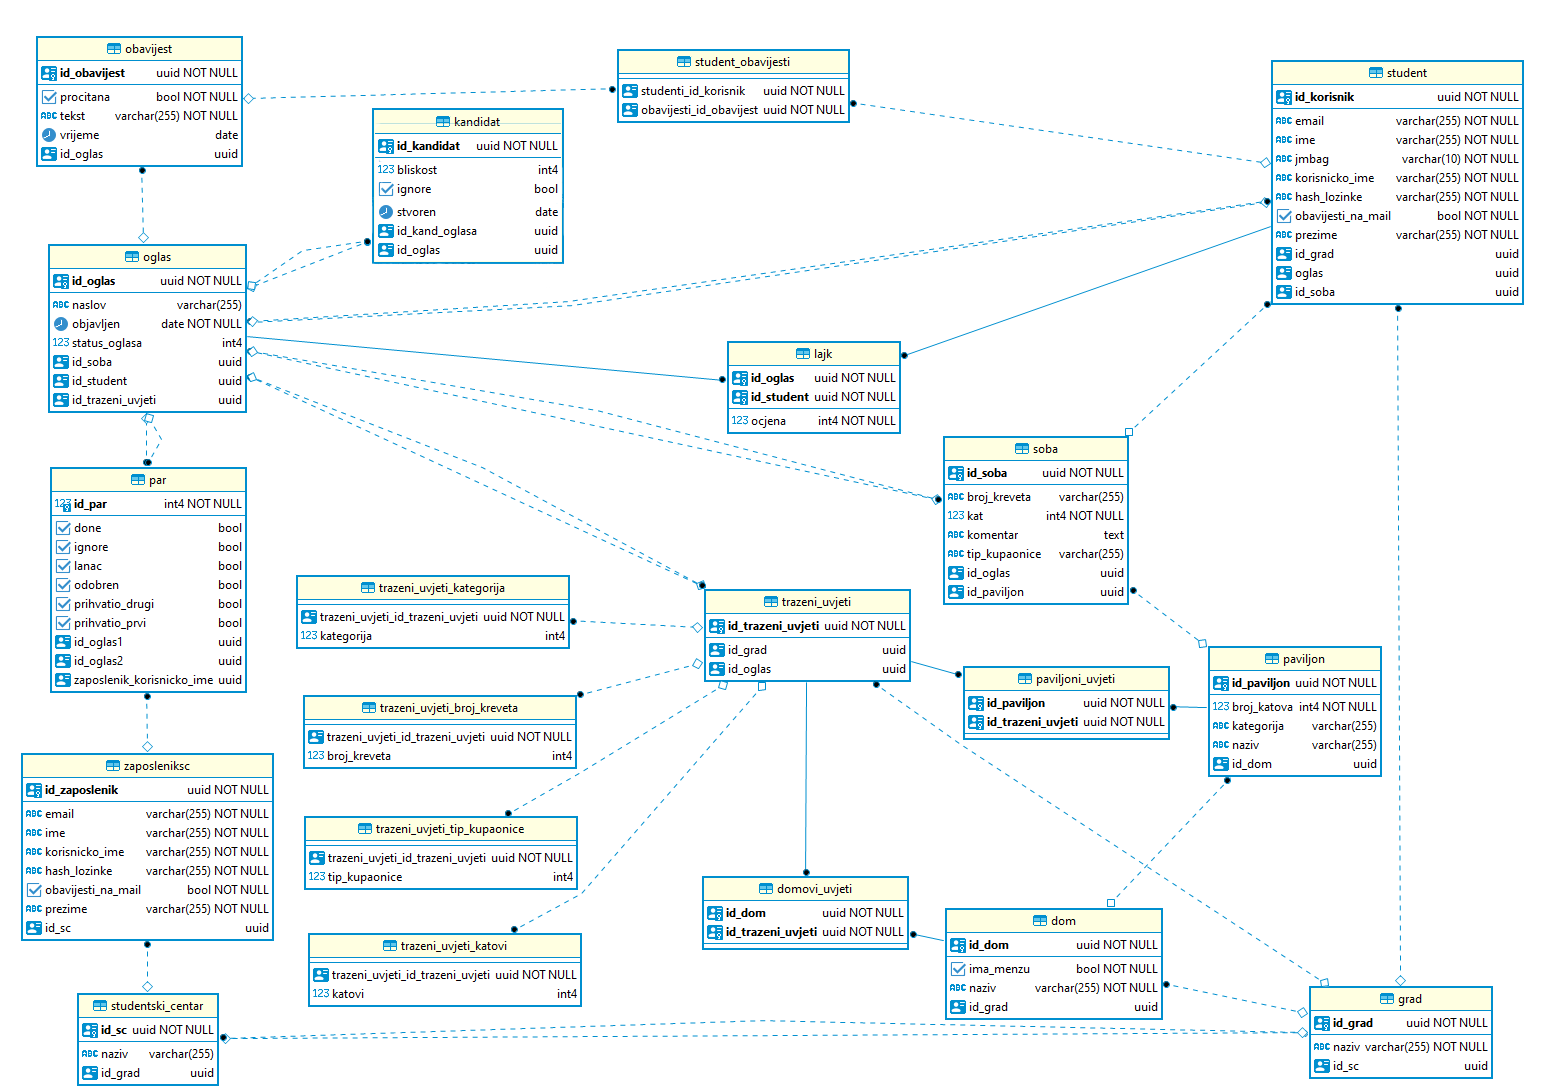
\includegraphics[scale=0.3]{dijagrami/baza.png} %veličina slike u odnosu na originalnu datoteku i pozicija slike
		\centering
		\caption{ER dijagram baze podataka}
		\label{fig:er}
	\end{figure}
	
	\eject
	
			
			
		\section{Dijagram razreda}
		
			Na slikama su prikazani razredi backenda. Na slici 4.4. prikazani su razredi Modela. Modeli opisuju entitete u bazi podataka. Na slici 4.5. prikazani su dijelovi Kontroler, Servis i Repozitorij. Kontroler AuthController manipulira s KorisnikDTO što je \textit{Data transfer object}(DTO) kojeg šaljemo na frontend kako bi mogli pamtiti trenutnog korisnika. Varijable KorsnikDTOa su dohvaćene metodama iz razreda Model.
			Kontroleri također pozivaju servise. Servisi obavljaju logiku aplikacije te za to koriste podatke iz razreda Model. Kontroleri i servisi pozivaju Repozitorij. To su sučelja koja nasljeđuju sučelje JpaRepository koje ima ugrađene metode za dohvat i spremanje podataka u bazu. Na slici 4.6. prikazan je dio Security. Razrede iz dijela Security pozivaju kontroleri za autentikaciju podataka.
		
			\begin{figure}[H]
				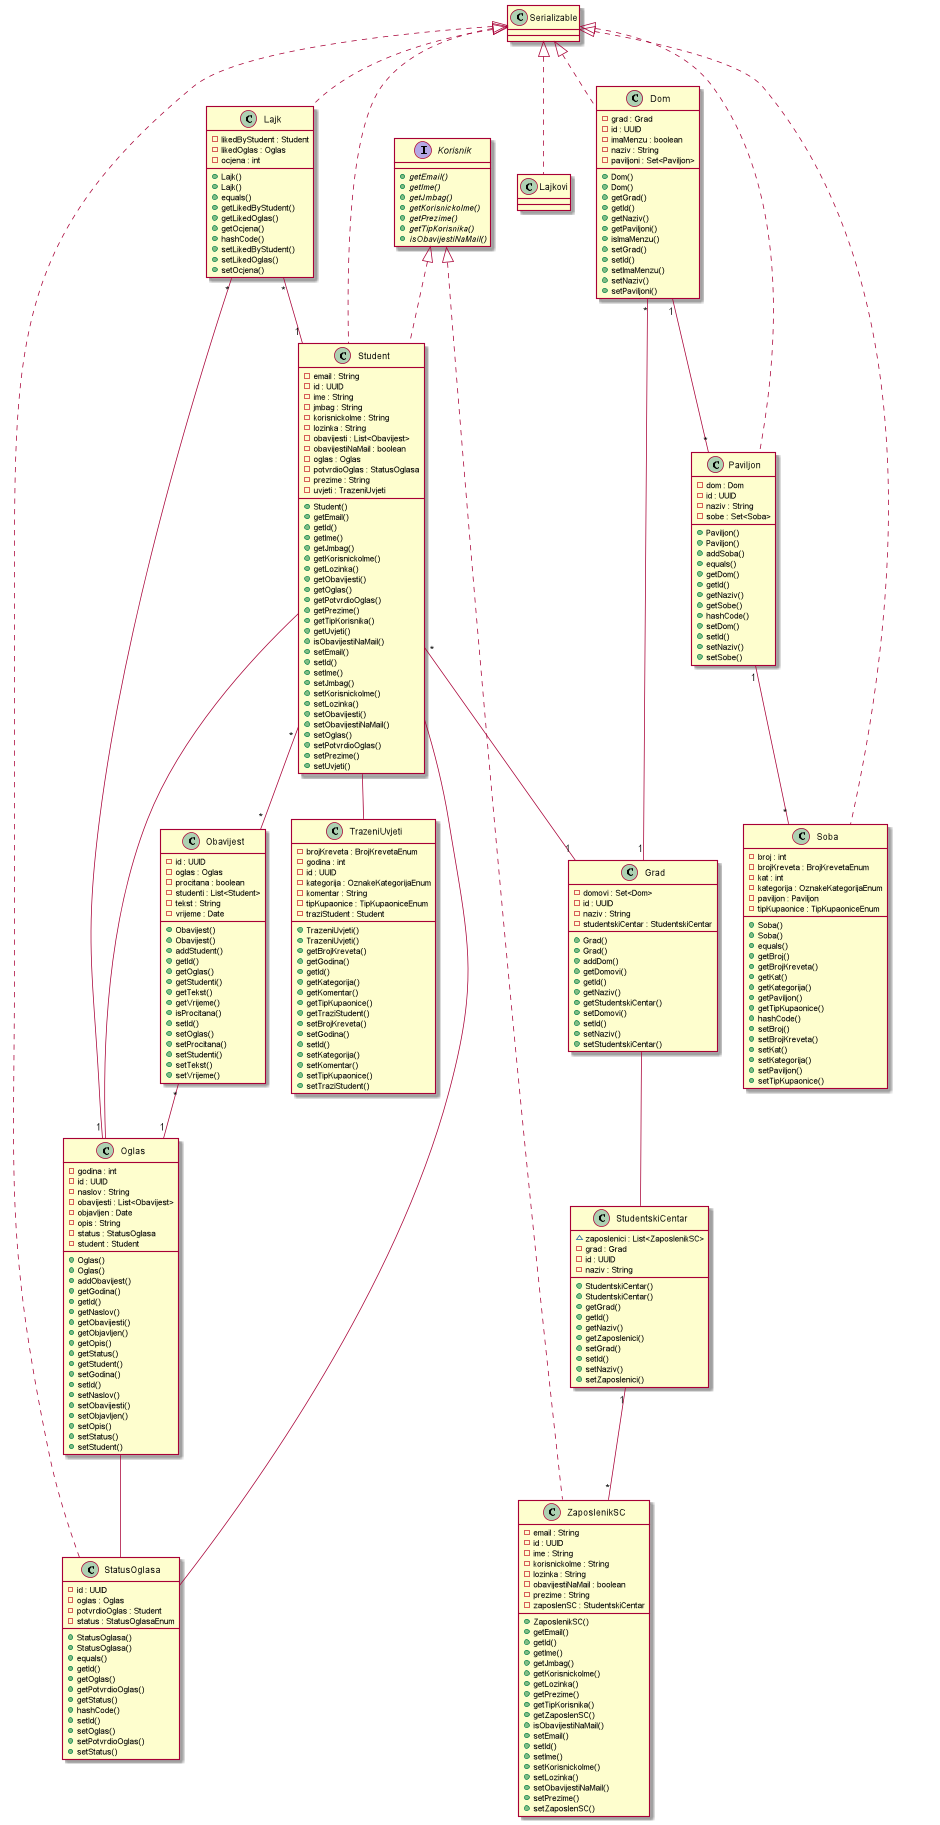
\includegraphics[scale=0.35]{dijagrami/model.png} %veličina slike u odnosu na originalnu datoteku i pozicija slike
				\centering
				\caption{Dijagrami razreda - dio Model}
				\label{fig:model}
			\end{figure}
		
			\begin{figure}[H]
				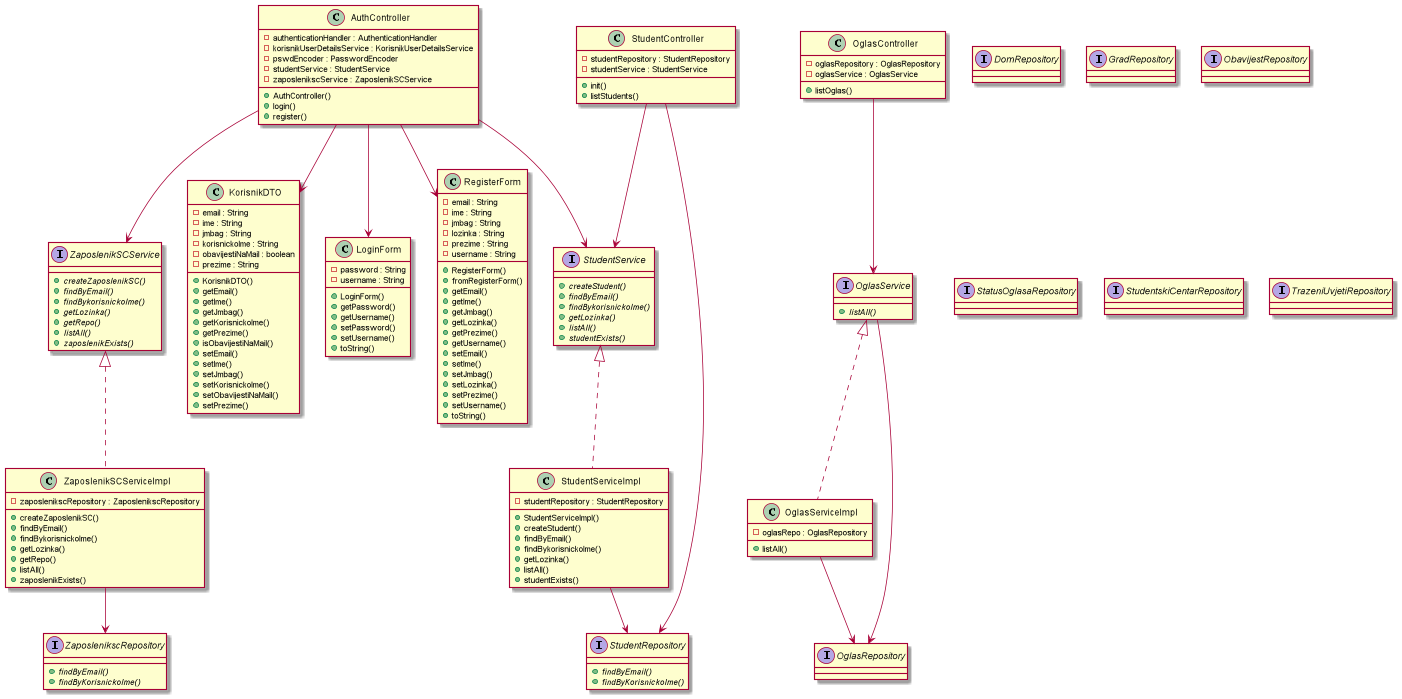
\includegraphics[scale=0.4]{dijagrami/controller.png} %veličina slike u odnosu na originalnu datoteku i pozicija slike
				\centering
				\caption{Dijagrami razreda - dio Kontroler, Servis i Repozitorij}
				\label{fig:controller}
			\end{figure}
		
			\begin{figure}[H]
				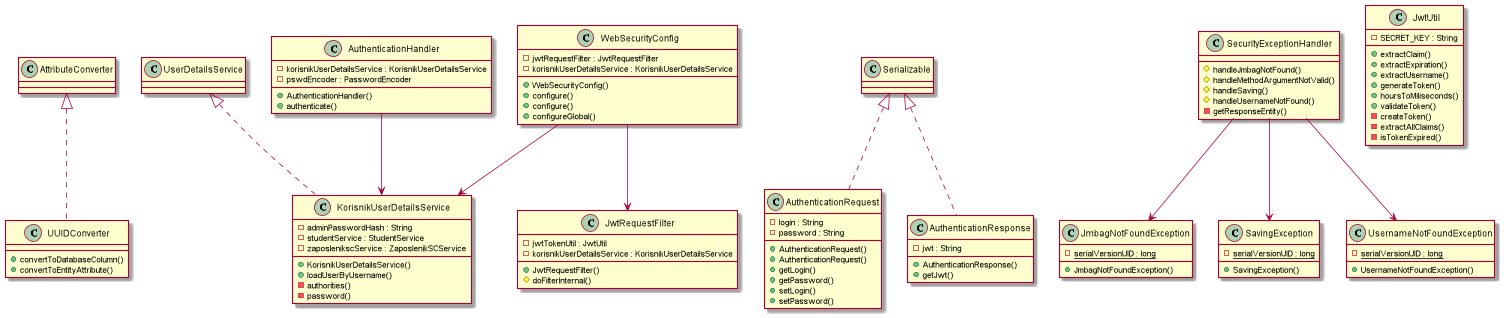
\includegraphics[scale=0.4]{dijagrami/security.png} %veličina slike u odnosu na originalnu datoteku i pozicija slike
				\centering
				\caption{Dijagrami razreda - dio Security}
				\label{fig:security}
			\end{figure}
		
		\eject
		
		\section{Dijagram stanja}
		
		
		Dijagram stanja ponašajni je UML dijagram koji opisuje dinamično ponašanje nekog dijela sustava prikazom konačnog broja stanja objekata te prijelaze između stanja koji su potaknuti događajima. Na dijagramu na slici 4.7 prikazan je dijagram stanja za prijavljenog korisnika. Kada se korisnik prijavi (ili registrira) prikazuje mu se početna stranica na kojoj su mu vidljivi svi oglasi i oglasi koji odgovaraju njegovim kriterijima, ako ih je postavio. Za svaki oglas korisnik može vidjeti dodatne informacije o sobi. Klikom na "Profil" prikazuju se svi podaci. Korisnik te podatke može ažurirati (osim podatka JMBAG te korisničkog imena). Također može izbrisati svoj profil. Klikom na ikonu zvona korisnik u padajućem izborniku može vidjeti nepročitane i pročitane obavijesti (ili poruku da nema obavijesti). Ako korisnik prethodno nije unio podatke o svojoj sobi, klikom na "Oglasi" prikazuje mu se forma za ponudu sobe u kojoj upisuje podatke o svojoj sobi. Nakon potvrde unosa prikazuje mu se i dodatna forma za traženje sobe u kojoj navodi tražene kriterije. Ako je korisnik već bio unio informacije o svojoj sobi, klikom na "Oglasi" odmah mu se prikazuju obje forme. Također, korisnik može mijenjati podatke i o svojoj sobi i o traženim kriterijima. Promjene se spremaju klikom na "Spremi promjene" na formama.
		\begin{figure}[H]
			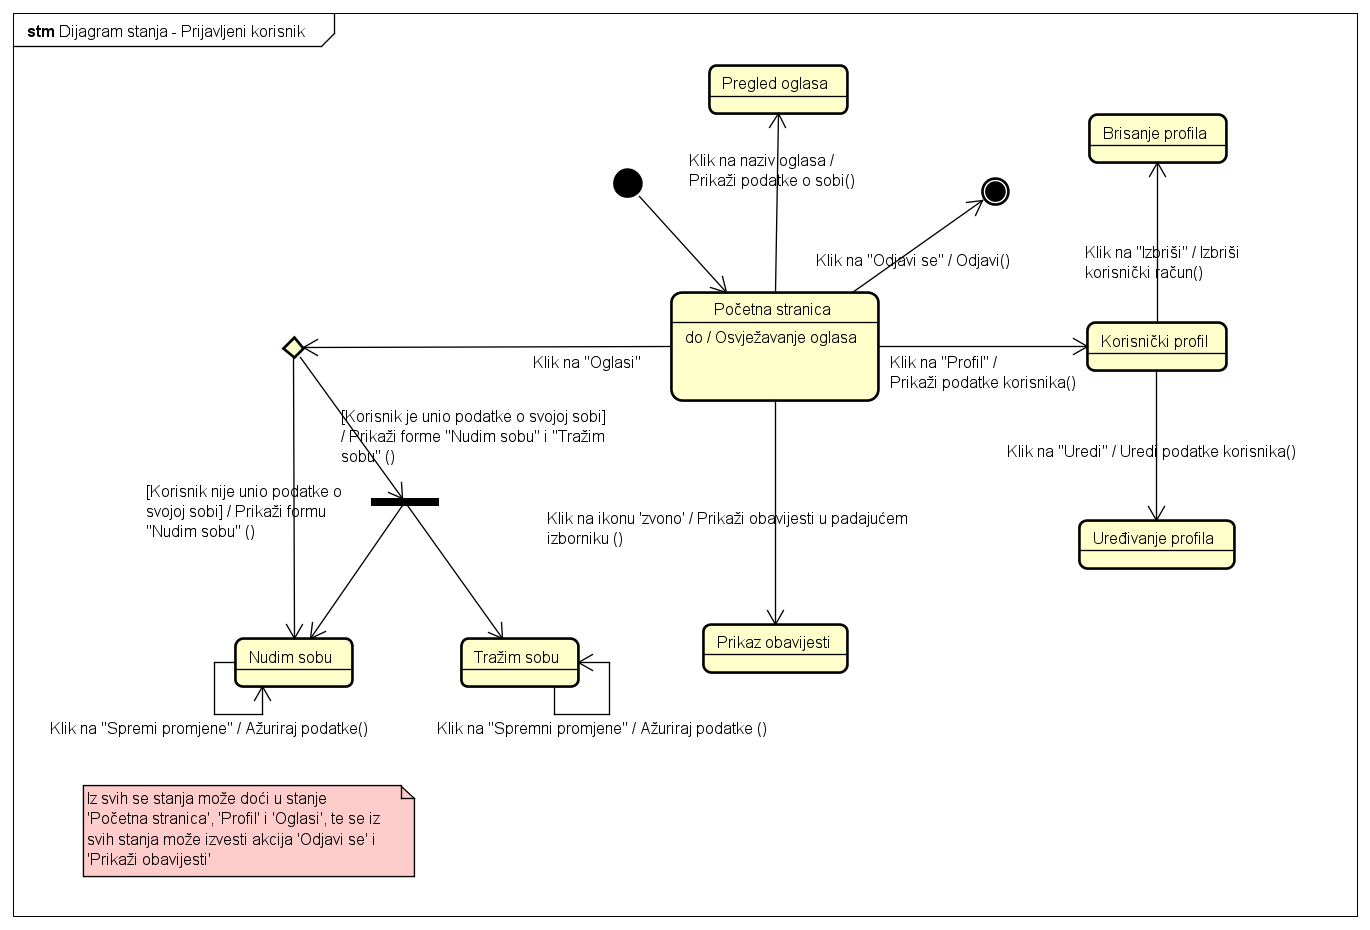
\includegraphics[scale=0.4]{dijagrami/dijagramStanja} %veličina slike u odnosu na originalnu datoteku i pozicija slike
			\centering
			\caption{Dijagram stanja}
			\label{fig:dijagramStanja}
		\end{figure}
		
		
		\eject 
		
		\section{Dijagram aktivnosti}
		
		\begin{figure}[H]
			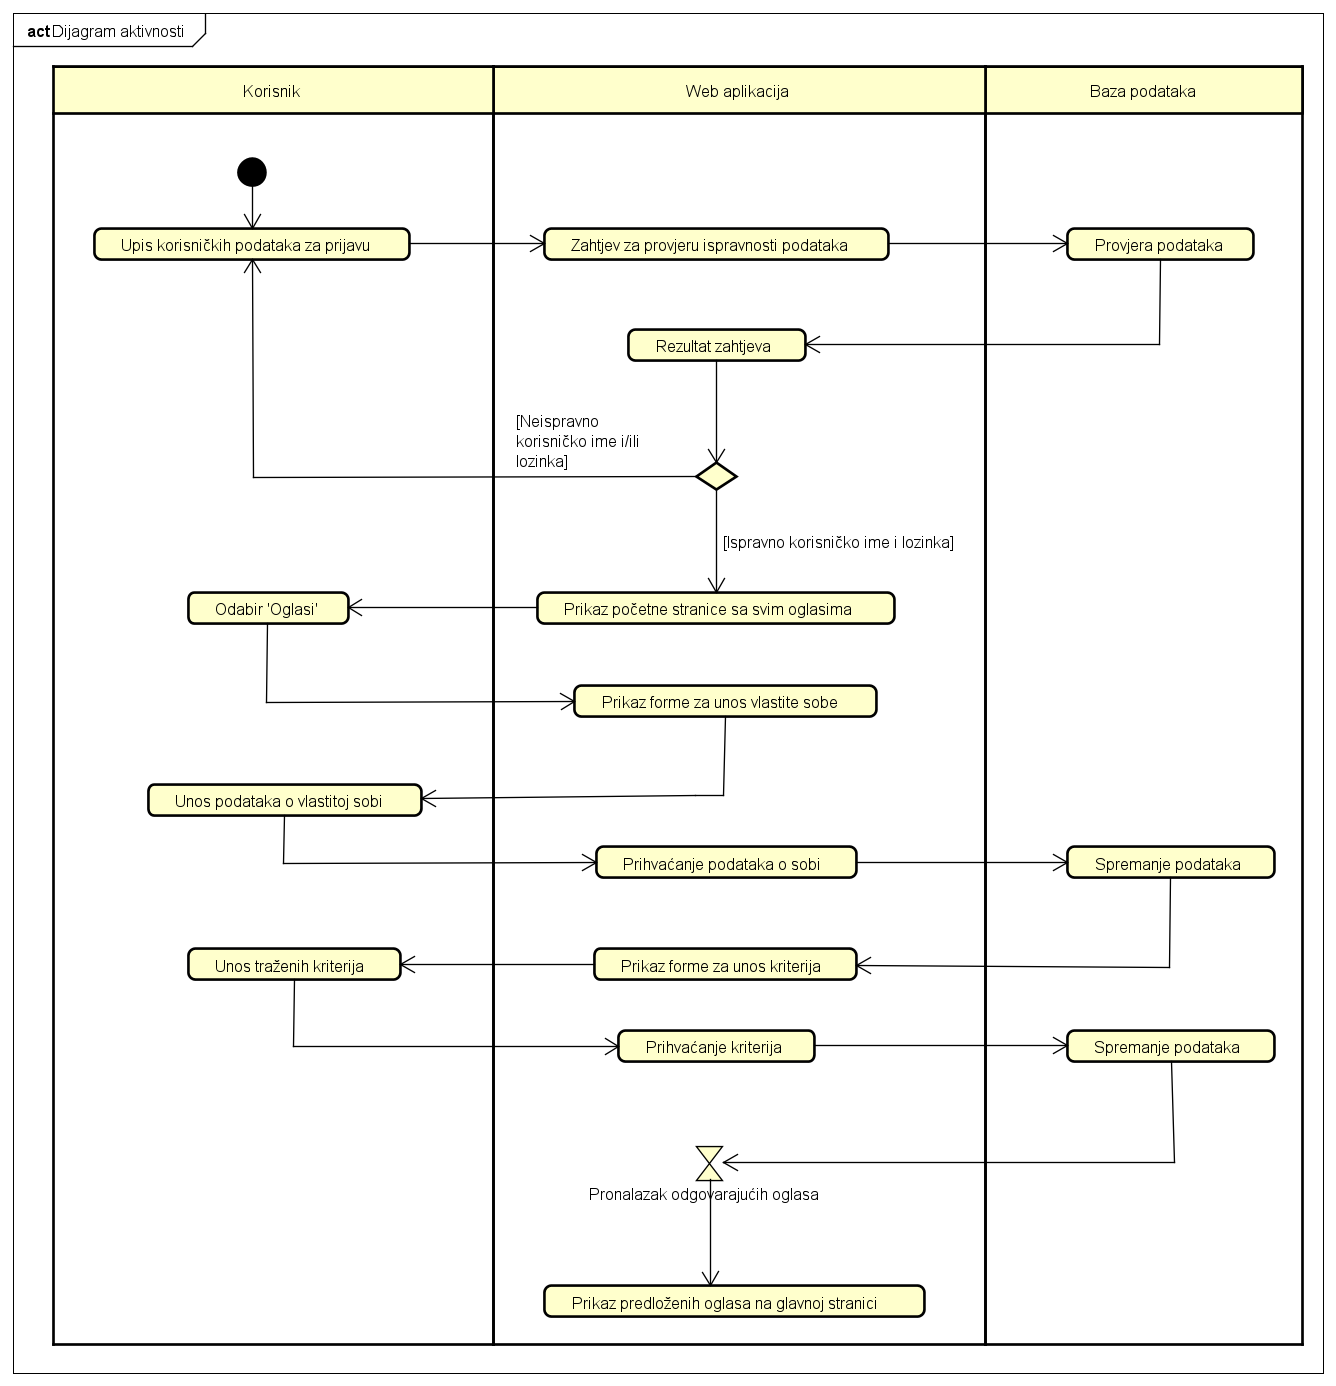
\includegraphics[scale=0.4]{dijagrami/dijagramAktivnosti} %veličina slike u odnosu na originalnu datoteku i pozicija slike
			\centering
			\caption{Dijagram aktivnosti}
			\label{fig:dijagramAktivnosti}
		\end{figure}
		
		\eject
		\section{Dijagram komponenti}
		
		
		
		\begin{figure}[H]
			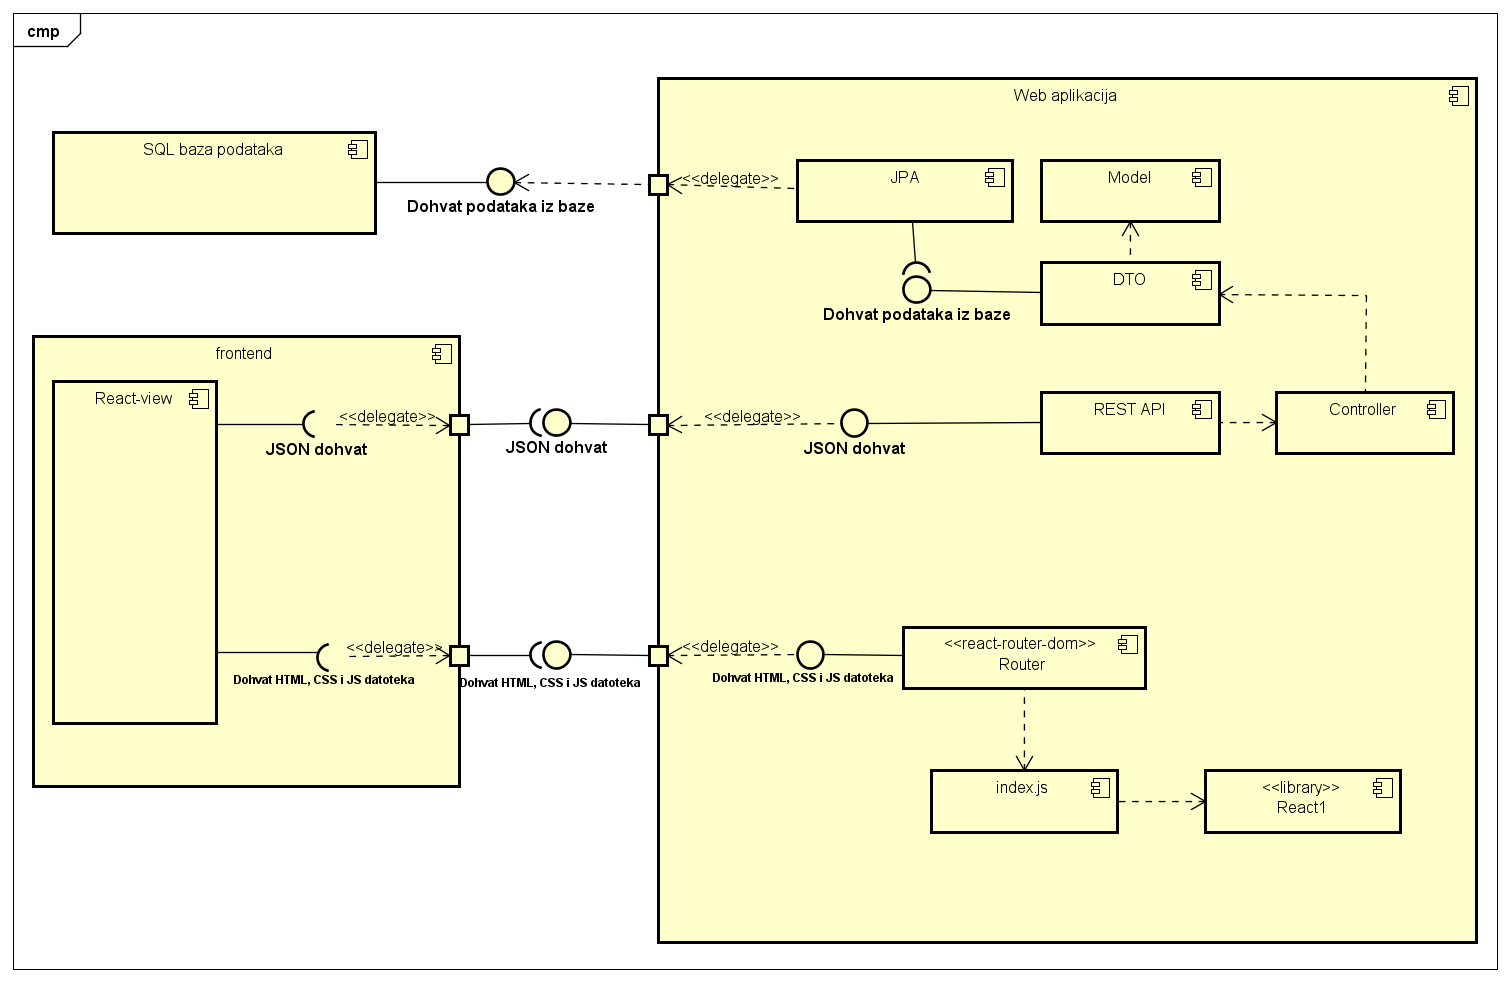
\includegraphics[scale=0.4]{dijagrami/dijagramKomponenti} %veličina slike u odnosu na originalnu datoteku i pozicija slike
			\centering
			\caption{Dijagram komponenti}
			\label{fig:dijagramKomponenti}
		\end{figure}
		
		
